\documentclass[tikz]{standalone}
% ------- TikZ Preamble -------
\RequirePackage{tikz}

\usetikzlibrary{
    spath3,
    intersections,
    arrows,
    knots,
    calc,
    hobby,
    decorations.pathreplacing,
    shapes.geometric,
     decorations.markings,
    decorations.pathmorphing,
    tikzlings}

% ------- Shared styles (from your preamble) -------
\tikzset{
    knot diagram/every strand/.append style={ultra thick, black},
%               every path/.style={black,line width=2pt},
%               every node/.style={transform shape,knot crossing,inner sep=1.5pt},
%               every knot/.style={line cap=round,line join=round,very thick},
%               strand/.style={line cap=round,line join=round,line width=3pt,draw=black},
%               over/.style={preaction={draw=white,line width=6.5pt}},
%               sst/ring A/.style={draw=black, line width=3pt},
%               sst/ring B/.style={draw=black,  line width=3pt},
%               sst/ring C/.style={draw=black, line width=3pt},
}

% ------- Guides toggle -------
\newif\ifsstguides
\sstguidestrue

% ------- Helper: label & skeleton for points P1..Pn -------
\newcommand{\SSTGuidesPoints}[2]{% #1=basename (e.g. P), #2=last index
  \ifsstguides
    \foreach \i in {1,...,#2}{
      \fill[blue] (#1\i) circle (1.2pt);
      \node[blue,font=\scriptsize,above] at (#1\i) {\i};
    }
    \draw[gray!40, dashed]
    \foreach \i [remember=\i as \lasti (initially 1)] in {2,...,#2,1} { (#1\lasti)--(#1\i) };
  \fi
}


% ------------------------------------------------------------
% \doubletwist{(A)}{(B)}{amplitude}{pitch}{line width}{color1}{color2}
%  - amplitude: lateral excursion of each strand [cm]
%  - pitch:     axial distance per full 360° twist [cm]
%  - line width: thickness of each colored strand
%  - colors:    e.g., red, blue, teal!70!black, etc.
% ------------------------------------------------------------
\newcommand{\doubletwist}[7]{%
% compute length (\n1) and angle (\n2)
    \path let \p1=#1, \p2=#2,
            \n1={veclen(\x2-\x1,\y2-\y1)},
\n2={atan2(\y2-\y1,\x2-\x1)} in
coordinate (S) at (#1);
\begin{scope}[shift={(S)}, rotate=\n2]
    % optional light guide (centerline)
\draw[gray!30, line width=0.6pt] (0,0) -- (\n1,0);
% strand 1
\draw[line width=#5, draw=#6]
plot[samples=250, domain=0:\n1] (\x,  {#3*sin(360*\x/#4)});
% strand 2 (phase-shifted by 180°)
\draw[line width=#5, draw=#7]
plot[samples=250, domain=0:\n1] (\x, -{#3*sin(360*\x/#4)});
\end{scope}%
}




\begin{document}

\begin{tikzpicture}[use Hobby shortcut, line cap=round, line join=round, scale=1.0]

% ---------------- parameters you can tune ----------------
\def\Amp{0.07}          % normal offset amplitude of each strand
\def\Turns{6}           % number of twist periods around the full loop
\def\Samples{80}       % number of sample points per strand (>= 80 recommended)
\def\Wth{2.5pt}         % line width of each colored strand
\def\ClrA{blue!80!black}
\def\ClrB{red!75!black}

% ---------------- your centerline control points ----------------
\coordinate (P1) at (-2.0,-2.0);  % start/close
\coordinate (P2) at (-2.0, 2.0);
\coordinate (P3) at ( 1.0,-0.5);
\coordinate (P4) at (-1.0,-0.5);
\coordinate (P5) at ( 2.0, 2.0);
\coordinate (P6) at ( 2.0,-2.0);
\coordinate (P7) at (-1.0, 0.5);
\coordinate (P8) at ( 1.0, 0.5);
\coordinate (P9) at (-2.0,-2.0);  % = P1

\def\KPATH{([closed] P1)..(P2)..(P3)..(P4)..(P5)..(P6)..(P7)..(P8)..(P9)}

% ---------------- helper: build strand coordinates along the path ----------------
% Makes coordinates A0..AN or B0..BN at normal offsets +/-Amp*sin(2π*Turns*s + phase)
% Local mark frame: x = tangent, y = left normal; so (0, yoffset) is a clean normal offset.
\newcommand{\MakeStrandCoords}[5]{%
% #1 = path macro, #2 = N samples, #3 = amplitude, #4 = turns, #5 = prefix
\pgfmathtruncatemacro{\Ns}{#2}
% phase = 0 for strand A, 0.5 for strand B (half period shift)
\def\Phase{0}%
\ifx#5B\def\Phase{0.5}\fi
\foreach \i in {0,...,\Ns}{%
\pgfmathsetmacro{\s}{\i/\Ns}%
\pgfmathsetmacro{\y}{#3*sin(360*(#4*\s + \Phase))}%
% place a coordinate at position s, offset \y along local normal
\path[
postaction={
decorate,
decoration={markings, mark=at position \s with {\coordinate (#5\i) at (0,\y);}}
}
] #1;%
}%
}

% Build both strands' coordinates
\MakeStrandCoords{\KPATH}{\Samples}{\Amp}{\Turns}{A}
\MakeStrandCoords{\KPATH}{\Samples}{\Amp}{\Turns}{B}

% ---------------- draw with proper crossing logic ----------------
\begin{knot}[
consider self intersections,
ignore endpoint intersections=true,
clip width=6pt, clip radius=3pt,
flip crossing/.list={2,4,6,8,10,12,14} % adjust to your preferred over/under
]
% Strand A (blue)
\strand[draw=\ClrA, line width=\Wth]
(A0) \foreach \i in {1,...,\Samples} { .. (A\i) } -- cycle;

% Strand B (red), half-period shifted (opposite side)
\strand[draw=\ClrB, line width=\Wth]
(B0) \foreach \i in {1,...,\Samples} { .. (B\i) } -- cycle;
\end{knot}

% (Optional) faint dashed centerline for reference:
% \draw[gray!40, dashed, line width=0.5pt] \KPATH;

\end{tikzpicture}


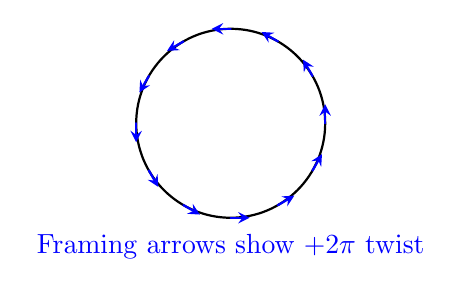
\begin{tikzpicture}[line cap=round, line join=round, scale=1.2]
% Base circle
\draw[thick] (0,0) circle(1);

% Twist arrows (+2π): evenly spaced along circle
\foreach \angle in {0,30,...,330}{
    \draw[->,>=stealth,blue,thick]
    ({cos(\angle)},{sin(\angle)}) -- ++({cos(\angle+90)*0.2},{sin(\angle+90)*0.2});
}

\node[blue] at (0,-1.3) {Framing arrows show +2$\pi$ twist};

\end{tikzpicture}

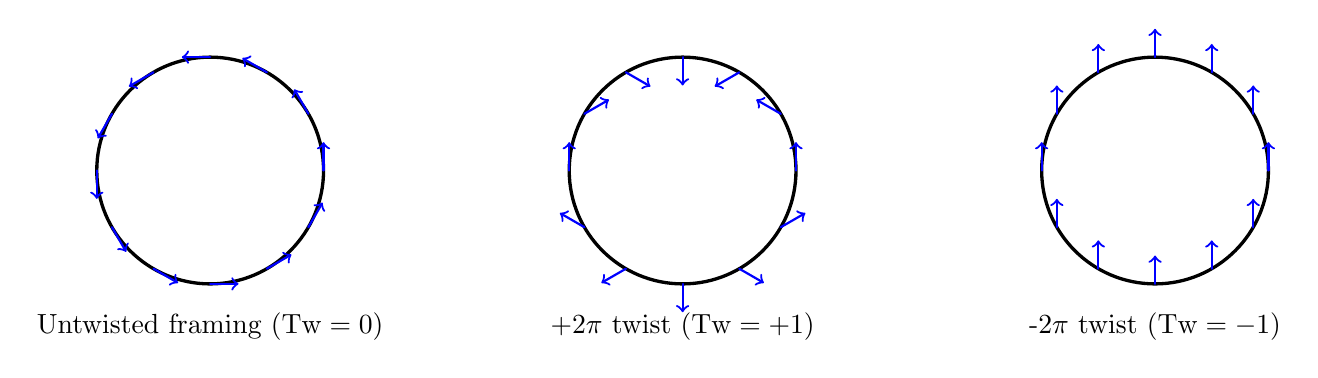
\begin{tikzpicture}[line cap=round, line join=round, scale=1.2]

% ---------- helper: draw a framed circle with a chosen arrow field ----------
% \framedcircle{center}{radius}{label}{mode}
%   mode = 0 : untwisted (arrows tangent)
%   mode = +1: +2pi twist (extra +1 rotation of arrows along the loop)
%   mode = -1: -2pi twist (extra -1 rotation of arrows along the loop)
\newcommand{\framedcircle}[4]{%
    \begin{scope}[shift={#1}]
    % centerline
    \draw[very thick] (0,0) circle (#2);
    % framing arrows along the circle
    \foreach \ang in {0,30,...,330}{
        % point on circle
        \pgfmathsetmacro{\cx}{#2*cos(\ang)}
        \pgfmathsetmacro{\cy}{#2*sin(\ang)}
        % base tangent direction (degrees): \ang+90
        % add extra twist: +\ang for +2pi, -\ang for -2pi, +0 for untwisted
        \ifnum#4=0
        \pgfmathsetmacro{\dir}{\ang+90}            % untwisted
        \else\ifnum#4=1
        \pgfmathsetmacro{\dir}{2*\ang+90}          % +2pi
        \else
                 \pgfmathsetmacro{\dir}{90}                 % -2pi (tangent minus one turn)
        \fi\fi
        % arrow length
        \def\alen{0.30}
        % draw arrow
        \draw[->,thick,blue]
        (\cx,\cy) -- ++({\alen*cos(\dir)},{\alen*sin(\dir)});
    }
% label
    \node[below=7pt] at (0,-#2) {#3};
    \end{scope}%
}

% ---------- three panels ----------
\framedcircle{(-5,0)}{1.2}{Untwisted framing ($\mathrm{Tw}=0$)}{0}
\framedcircle{(0,0)}{1.2}{+$2\pi$ twist ($\mathrm{Tw}=+1$)}{1}
\framedcircle{(5,0)}{1.2}{-$2\pi$ twist ($\mathrm{Tw}=-1$)}{-1}

\end{tikzpicture}
\end{document}

